
\thispagestyle{empty}
\section{Backpropagation}\label{sec:backpropagation}   

\vspace{1cm}
\begin{tcolorbox}[title={Inhalte der \textit{Backpropagation}}]
  \begin{quotation}\noindent
    Es wird ein Algorithmus gesucht, der die Wege ermittelt, welche einen stärkeren Einfluss auf den Output haben. Ebenso sollen diese Verbindungen dann gestärkt oder abgeschwächt werden.
    Dieses Kapitel erläutert, wie durch die Backpropagation ein neuronales Netz angepasst werden kann, um einen gewünschten Output zu erzielen. 
  \end{quotation}
  \begin{itemize}
    \item Was ist eine geeignete Verlustfunktion?
    \item Wie lernen Neuronale Netze?
    \item Grundidee Backpropagation
    \item Wie funktioniert der Backpropagation-Algorithmus
  \end{itemize}
\end{tcolorbox}

\subsection{Was ist eine geeignete Verlustfunktion?}\label{subsec:backpropagation:verlustfunktion}
Die Verlustfunktion wird genutzt um den Fehler eines neuronalen Netzes zu berechnen. Dieser Fehler gibt an, 
wie sehr die wirklichen Ausgabewerte des neuronalen Netzes nach Eingabe eines Trainingsdatensatzes von den gewollten Ausgabewerten abweichen. 
\bigbreak\noindent
Eine weitverbreitete Verlustfunktion ist der sogenannte Mean Squared Error (MSE), bei dem der Durchschnitt der quadrierten Fehler berechnet wird.
Bei Anwendung auf neuronale Netze lässt sich diese Funktion wie folgt ausdrücken:

\begin{eqnarray}  
  C(w,b) = \frac{1}{2n} \sum_x \| y(x) - a\|^2.
\end{eqnarray}

\noindent
In dieser Gleichung steht $w$ für die Gesamtheit aller Gewichte im neuronalen Netz, während $b$ alle Biases repräsentiert.
$n$ bezeichnet die Anzahl der Trainingsdatensätze und $y(x)$ ist der Vektor der Soll-Werte nach einem einzigen Trainingsbeispiel.
Schließlich ist $a$ der Vektor der tatsächlichen Ausgabewerte. 
\bigbreak\noindent
Wichtige Eigenschaften der MSE Verlustfunktion sind zum einen, dass sie niemals negativ wird, da jeder Term der Funktion positiv ist.
Außerdem sieht man recht einfach, dass $C(w, b) \approx 0$ gilt, wenn die die Soll-Werte ungefähr gleich den tatsächlichen Ausgabewerten sind.
\bigbreak\noindent
Es wird der durchschnittliche Fehler über \textbf{alle} Trainingsbeispiele berechnet. 
Es gibt Methoden, bei denen der Fehler nur für ausgewählte Teilgruppen (sog. Batches) von Trainingsbeispielen berechnet wird (Batch-Methode). 
Diese Vorgehensweise kann die Laufzeit des Backpropagation-Algorithmus verbessern, wird in diesem Text jedoch nicht weiter vertieft.
% TODO: Quelle angeben: http://neuralnetworksanddeeplearning.com/chap1.html#learning_with_gradient_descent

\subsection{Wie lernen Neuronale Netze?}\label{subsec:backpropagation:lernen_nn}
Da wir nun eine Verlustfunktion kennen, welche den Fehler eines neuronalen Netzes bestimmt, kann man eben jene
Verlustfunktion nutzen um das neuronale Netz lernen zu lassen. Der Ausgabewert der Verlustfunktion hängt sowohl von allen Weights $w$ 
als auch von allen Biases $b$ des neuronalen Netzes ab. Nun sucht man die konkreten Werte für die Weights und Biases, damit die 
Verlustfunktion so klein wie möglich wird. Dies tut man mit dem bereits oben beschriebenen Gradientenverfahren. Man braucht also den 
negativen Gradientenvektor der Verlustfunktion.

\subsection{Grundidee Backpropagation}\label{subsec:backpropagation:grundiee}
Backpropagation stellt einen effizienten Algorithmus zur Berechnung dieses komplexen Gradientenvektors dar, den wir benötigen, um den Fehler in einem neuronalen Netzwerk zu minimieren.
Der Fehler an der Ausgabeschicht muss durch das gesamte Netz propagiert werden, um die Gewichte und Biaswerte entsprechend anzupassen.
Für jedes Gewicht und jeden Biaswert möchten wir bestimmen, wie stark der Fehler von diesem abhängt. 
Hierbei werden die partiellen Ableitungen verwendet, die die Sensitivität einer Funktion in Bezug auf eine Änderung einer bestimmten Variable messen.
Konkret suchen wir nach den Werten von $\frac{\partial C}{\partial w_{jk}^{l}}$ und $\frac{\partial C}{\partial b_{j}^{l}}$, die partiellen Ableitungen der Kostenfunktion (C) nach den Gewichten ($w_{jk}^{l}$) und Biaswerten ($b_{j}^{l}$).

\subsection{Wie funktioniert der Backpropagation-Algorithmus}\label{subsec:backpropagation:fehlerrueckfuehrung}
Für die Erklärung des Backpropagation-Algorithmus nehmen wir folgendes neuronales Netz an:
\begin{figure}[H]
  \centering
  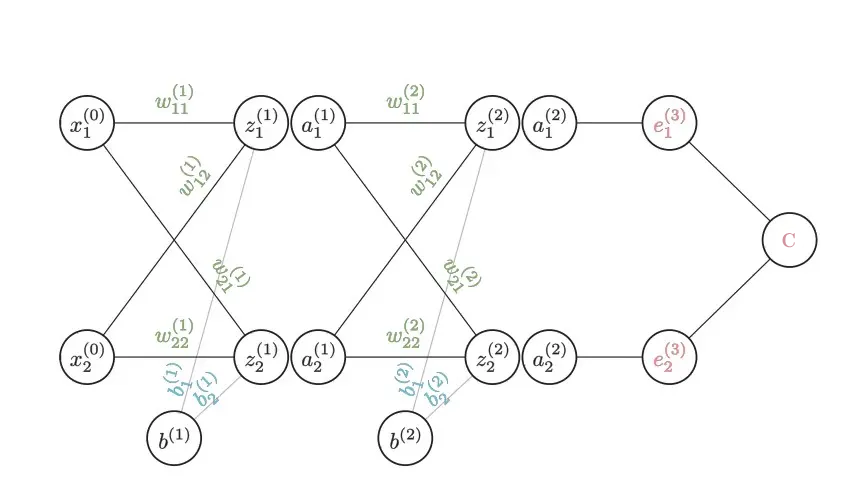
\includegraphics[width=0.5\textwidth]{Sources/04-05_backprop_nn_example.png}
  \caption{Hier Quelle angeben}
\end{figure}
\noindent
Der gesamte Fehler $C$ wurde in der Abbildung auf die zwei Output-Neuronen über $e_1^{(3)}$ und $e_2^{(3)}$ aufgeteilt.
Außerdem wurde jedes Hidden-Neuron in seine gewichtete Summe $z$ und seine Aktivierungsfunktion $a$ aufgeteilt.
Zuerst muss man sich überlegen, wie man die Weights / Biases, welche in die Output-Schicht einfließen anpasst.
Wenn man nun beispielsweise ausrechnen möchte welchen Einfluss das Gewicht $w_{11}^{(2)}$ auf den Fehler C hat, dann muss man 
$\frac{\partial C}{\partial w_{11}^{(2)}}$ berechnen. Hierfür macht es Sinn, dass man sich anschaut wie das Weight $w_{11}^{(2)}$ in den Fehler C einfließt.
Das Gewicht $w_{11}^{(2)}$ geht nur in den Teilfehler $e_1$ ein, daher muss man auch nur diesen betrachten.
\begin{flalign*}  
  e_{1}^{(3)} &= (y(x) - a_1^{(2)})^2\\
  a_{1}^{(2)} &= \sigma(z_{1}^{(2)})\\
  z_{1}^{(2)} &= w_{11}^{(2)} * a_{1}^{(1)} + w_{12}^{(2)} * a_{2}^{(1)} + b_1^{(2)}\\
  \Rightarrow e_{1}^{(3)} &= (y(x) - \sigma(w_{11}^{(2)} * a_{1}^{(1)} + w_{12}^{(2)} * a_{2}^{(1)} + b_1^{(2)}))^2
\end{flalign*}
\noindent
Möchte man nun die oben genannte partielle Ableitung ausrechnen, dann macht man sich die Kettenregeln zu Nutze und es gilt: 
\begin{align*}  
  \frac{\partial C}{\partial w_{11}^{(2)}} = \frac{\partial e_1^{(3)}}{\partial a_1^{(2)}}\frac{\partial a_1^{(2)}}{\partial z_{1}^{(2)}}\frac{\partial z_{1}^{(2)}}{\partial w_{11}^{(2)}}
\end{align*}
\noindent
Diesen Schritt würde man für jedes Weight ausführen, welches in ein Output-Neuron einfließt.
Anstatt jede partielle Ableitung einzeln aufzuschreiben macht man sich das Hadamard-Produkt zu Nutze um effizient alle partiellen
Ableitungen dieser Weights zu berechnen:
\begin{align*}
  \renewcommand{\arraystretch}{1.5}
  \begin{bmatrix}
    \frac{\partial C}{\partial w_{11}^{(2)}} & \frac{\partial C}{\partial w_{12}^{(2)}} \\
    \frac{\partial C}{\partial w_{21}^{(2)}} & \frac{\partial C}{\partial w_{22}^{(2)}} \\
  \end{bmatrix} = 
  \begin{bmatrix}
    \frac{\partial e_1^{(3)}}{\partial a_1^{(2)}} \\
    \frac{\partial e_2^{(3)}}{\partial a_2^{(2)}}
  \end{bmatrix} \odot 
  \begin{bmatrix}
    \frac{\partial a_1^{(2)}}{\partial z_1^{(2)}} \\
    \frac{\partial a_2^{(2)}}{\partial z_2^{(2)}}
  \end{bmatrix} \odot
  \begin{bmatrix}
    \frac{\partial z_1^{(2)}}{\partial w_{11}^{(2)}} & \frac{\partial z_1^{(2)}}{\partial w_{12}^{(2)}} \\
    \frac{\partial z_2^{(2)}}{\partial w_{21}^{(2)}} & \frac{\partial z_2^{(2)}}{\partial w_{22}^{(2)}} \\
  \end{bmatrix}
  \renewcommand{\arraystretch}{1}
\end{align*}
\noindent
Die zwei linken Vektoren des Hadamard-Produkts werden im folgenden noch zu einem $\delta$ Term zusammengefasst, da diese in späteren 
Berechnungen öfters auftreten.
\begin{align*}
  \delta^{(L)} = \frac{\partial C}{\partial A^{(2)}} \odot \frac{\partial A^{(2)}}{\partial Z^{(2)}}\\
  \\
  \Rightarrow \frac{\partial C}{\partial W^{(2)}} = \delta^{(L)} \odot \frac{\partial Z^{(2)}}{\partial W^{(2)}}
\end{align*}
\noindent
Jetzt muss man sich noch anschauen wie man die Abhängigkeit des Fehlers eines tiefer liegenden Weights / Biases 
berechnet, z.B. $\frac{\partial C}{\partial w_{11}^{(1)}}$. Die Grundidee bleibt die selbe, jedoch können nun mehrere Pfade vom gesamten Fehler 
zu diesem Weight führen. In diesem Fall addieren wir die Kettenregel-Terme beider Pfade zusammen, bis sie sich an einem Neuron treffen.
\begin{align*}  
  \frac{\partial C}{\partial w_{11}^{(1)}} = (\frac{\partial e_1^{(3)}}{\partial a_1^{(2)}}\frac{\partial a_1^{(2)}}{\partial z_1^{(2)}}\frac{\partial z_1^{(2)}}{\partial a_1^{(1)}} + \frac{\partial e_2^{(3)}}{\partial a_2^{(2)}}\frac{\partial a_2^{(2)}}{\partial z_2^{(2)}}\frac{\partial z_2^{(2)}}{\partial a_1^{(1)}})
  \frac{\partial a_1^{(1)}}{\partial z_1^{(1)}}\frac{\partial a_1^{(1)}}{\partial w_{11}^{(1)}}
\end{align*}
In dieser Gleichung sieht man nun auch die sich wiederholenden $\delta^{L}$ Terme.
\begin{align*}  
  \frac{\partial C}{\partial w_{11}^{(1)}} = (\delta_1^{L}\frac{\partial z_1^{(2)}}{\partial a_1^{(1)}} + \delta_2^{L}\frac{\partial z_2^{(2)}}{\partial a_1^{(1)}})
  \frac{\partial a_1^{(1)}}{\partial z_1^{(1)}}\frac{\partial a_1^{(1)}}{\partial w_{11}^{(1)}}
\end{align*}
\noindent
Auch diese Berechnung führen wir für jedes "tiefere" Weight (in dem Fall von der 1. zur 2. Schicht) aus. Durch Matrizen lässt sich diese Berechnung wiefolgt ausdrücken: 
\begin{align*}
  \renewcommand{\arraystretch}{1.5}
  \begin{bmatrix}
    \frac{\partial C}{\partial w_{11}^{(1)}} & \frac{\partial C}{\partial w_{12}^{(1)}} \\
    \frac{\partial C}{\partial w_{21}^{(1)}} & \frac{\partial C}{\partial w_{22}^{(1)}}
  \end{bmatrix} = \begin{bmatrix}
   \delta_1^L \\
   \delta_2^L
  \end{bmatrix}^T \cdot  
  \begin{bmatrix}
    \frac{\partial z_1^{(2)}}{\partial a_1^{(1)}} & \frac{\partial z_1^{(2)}}{\partial a_2^{(1)}}\\
    \frac{\partial z_2^{(2)}}{\partial a_1^{(1)}} & \frac{\partial z_2^{(2)}}{\partial a_2^{(1)}}
  \end{bmatrix} \odot 
  \begin{bmatrix}
    \frac{\partial a_1^{(1)}}{\partial z_1^{(1)}} \\
    \frac{\partial a_2^{(1)}}{\partial z_2^{(1)}}
  \end{bmatrix} \odot
  \begin{bmatrix}
   \frac{\partial z_1^{(1)}}{\partial w_{11}^{(1)}} && \frac{\partial z_1^{(1)}}{\partial w_{12}^{(1)}}\\
   \frac{\partial z_2^{(1)}}{\partial w_{21}^{(1)}} && \frac{\partial z_2^{(1)}}{\partial w_{22}^{(1)}}
  \end{bmatrix}
  \renewcommand{\arraystretch}{1.0}
\end{align*}
\begin{align*}
  \Rightarrow \frac{\partial C}{\partial W^{(1)}} = (\delta^L)^T \cdot \frac{\partial Z^{(2)}}{\partial A^{(1)}} \odot
  \frac{\partial A^{(1)}}{\partial Z^{(1)}} \odot \frac{\partial Z^{(1)}}{\partial W^{(1)}}
\end{align*}
\noindent
Die Berechnungen für die Bias-Werte sehen sehr ähnlich aus, daher werden diese hier nicht weiter ausgeführt.
Somit kommt man auf die allgemeinen Formeln für die Backpropagation: 
\begin{flalign*}
  \frac{\partial C}{\partial W^{(l)}} &= (\delta^{(l+1)})^T \cdot W^{(l+1)} \odot \frac{\partial A^{(l)}}{\partial Z^{(l)}} \odot X^{(l - 1)}\\
  \delta^{(L)} &= \frac{\partial C}{\partial A^{(L)}} \odot \frac{\partial A^{(L)}}{\partial Z^{(L)}}\\
  \frac{\partial C}{\partial B^{l}} &= \delta^l
\end{flalign*}
